\documentclass[11pt,a4paper]{article}
\usepackage[utf8]{inputenc}
\usepackage[margin=1in]{geometry}
\usepackage{amsmath,amssymb,amsfonts}
\usepackage{graphicx}
\usepackage{booktabs}
\usepackage{hyperref}
\usepackage{microtype}
\usepackage{subcaption}
\usepackage{cite}

\title{\textbf{EpiGraph: Dynamic Usage-Weighted Topology and Synaptic Consolidation for Multi-Hop Agentic Memory}}

\author{
  \textbf{Teja P.}\\
  \texttt{teja@antigravity.ai}
}

\date{\today}

\begin{document}

\maketitle

\begin{abstract}
As autonomous Large Language Model (LLM) agents are deployed across sustained, multi-session environments, conventional memory architectures suffer from three fundamental pathologies: (1) \textbf{Associative Blindness}, wherein flat dense vector indexes fail to traverse multi-hop relational dependencies across distant interaction sessions; (2) \textbf{Scaffolding Amnesia}, where standard wall-clock temporal decay rules aggressively erase foundational user identity and architectural constraints; and (3) \textbf{Static Topology Stagnation}, where existing graph-augmented retrieval systems treat network structure as immutable, ignoring real-time usage dynamics and task utility.

In this work, we propose \textbf{EpiGraph}, a biologically inspired, hierarchical hybrid memory architecture for autonomous agents. EpiGraph partitions memory operations into a low-latency streaming ingestion/retrieval ``Waking State'' and an asynchronous background ``Dreaming State'' consolidation cycle. We introduce three core theoretical contributions:
\begin{enumerate}
    \item \textbf{Usage-Modulated Personalized PageRank (U-PPR)}: A spreading activation algorithm where transition probabilities adapt via activity-dependent Hebbian plasticity, dynamically promoting persistent foundational entities into high-centrality \textbf{Epistemic Macro-Hubs (``God Nodes'')}.
    \item \textbf{Consolidation-Activated Topology Decay (CATD)}: A synaptic forgetting rule executed strictly off the read path that scales retention half-life by topological load-bearing weight rather than wall-clock time, protecting foundational scaffolding with a cold-start grace period.
    \item \textbf{Hierarchical Context Engineering}: A multi-leg retrieval pipeline fusing dense vectors, U-PPR graph traversal, and BM25 via dynamic intent-routed Reciprocal Rank Fusion (RRF).
\end{enumerate}
We evaluate EpiGraph locally across all 10 long-term multi-session conversations (496 evaluation QA pairs) in the \textbf{LoCoMo} benchmark. EpiGraph achieves a \textbf{+58.3\% relative improvement in Recall@1} (22.47\% vs. 14.19\%) and a \textbf{+25.9\% relative improvement in Recall@5} (40.79\% vs. 32.39\%) over dense vector RAG, while surpassing static graph RAG by more than $5\times$. On temporal reasoning, EpiGraph yields an \textbf{+18.11 percentage point gain} (63.60\% vs. 45.49\%). Longitudinal 90-day continuous deployment simulations prove that CATD achieves 100\% scaffolding retention where baseline temporal decay degrades to 60\%, all while maintaining sub-25ms retrieval latency.
\end{abstract}

\section{Introduction}

Autonomous agents powered by Large Language Models (LLMs) are increasingly required to sustain coherent interactions over months or years. While context window sizes have expanded substantially, simply concatenating past interaction histories into prompt contexts incurs quadratic attention computation, attention dilution, and the well-documented ``Lost-in-the-Middle'' phenomenon.

To provide persistent state across disjoint sessions, current systems predominantly rely on either:
\begin{itemize}
    \item \textbf{Flat Vector RAG}: Storing chunked dialogues in vector databases (e.g., HNSW indices) and retrieving top-$K$ chunks via cosine similarity.
    \item \textbf{OS-Inspired Virtual Memory}: Using explicit LLM tool calls to page memory chunks between context RAM and archival disk (e.g., MemGPT \cite{packer2023memgpt}).
    \item \textbf{Static Knowledge Graph RAG}: Extracting entity-relation triples into static knowledge graphs traversed via static Personalized PageRank (e.g., HippoRAG \cite{bernal2024hipporag}) or hierarchical Leiden communities (e.g., GraphRAG \cite{edge2024graphrag}).
\end{itemize}

Despite their strengths, these paradigms fail in continuous conversational agent deployments. Flat vector search cannot traverse associative multi-hop relationships that span across multiple sessions. Conversely, static graph architectures assume a fixed document corpus, ignoring the dynamic, living nature of agent-user conversations where entities frequently recur, mutate, or contradict prior assertions. Furthermore, naive temporal decay models suffer from \textbf{Scaffolding Amnesia}—erasing foundational user persona and system constraints simply because they are not discussed on a daily basis.

\paragraph{Contributions.} In this paper, we present \textbf{EpiGraph}, a unified framework that overcomes these limitations:
\begin{itemize}
    \item We formulate \textbf{Dynamic Hebbian Usage Plasticity} on memory graphs, where edge weights dynamically strengthen when co-retrieved during conversational tasks.
    \item We introduce \textbf{Usage-Modulated Personalized PageRank (U-PPR)} and mathematically define the emergence of \textbf{Epistemic Macro-Hubs (``God Nodes'')} that anchor multi-hop context expansion.
    \item We formulate \textbf{Consolidation-Activated Topology Decay (CATD)}, solving the Scaffolding Amnesia problem through load-bearing topological retention.
    \item We validate EpiGraph on the full 10-conversation, 496-question \textbf{LoCoMo} benchmark \cite{mahbub2024locomo}, demonstrating substantial gains across factual, temporal, and multi-session reasoning categories with sub-25ms query latency.
\end{itemize}

\section{Related Work}

\paragraph{Vector RAG and Score Incomparability.} Dense vector embeddings mapped into Hierarchical Navigable Small World (HNSW) graphs \cite{malkov2018hnsw} provide sub-millisecond similarity search. However, dense vectors struggle with exact keywords (e.g., error codes, IDs). While hybrid search incorporates Okapi BM25 \cite{robertson2009bm25}, raw vector distances and BM25 scores are fundamentally incomparable. Reciprocal Rank Fusion (RRF) \cite{cormack2009rrf} circumvents score normalization by aggregating ordinal ranks.

\paragraph{Graph-Augmented Agent Memory.} HippoRAG \cite{bernal2024hipporag} draws inspiration from the neurobiological Complementary Learning Systems (CLS) theory, using an OpenIE knowledge graph and Personalized PageRank \cite{page1999pagerank} as an associative hippocampal index. Microsoft GraphRAG \cite{edge2024graphrag} uses the Leiden/Louvain algorithm \cite{blondel2008louvain} to generate macro-summaries. However, both frameworks treat graphs as static indices over static corpora, lacking operational usage feedback, dynamic plasticity, or active pruning.

\paragraph{Long-Term Memory Benchmarks.} Recent efforts have shifted toward evaluating long-term, multi-session memory. The \textbf{LoCoMo} benchmark \cite{mahbub2024locomo} evaluates factual recall, temporal reasoning, and multi-hop inference across up to 35 conversational sessions. \textbf{LongMemEval} \cite{wu2025longmemeval} and \textbf{MemoryArena} \cite{memoryarena2026} evaluate knowledge updates and closed-loop decision making.

\section{The EpiGraph Architecture}

EpiGraph implements a dual-brain architecture decoupling fast-path interaction from slow-path consolidation:

\subsection{Waking State: Ingestion and Retrieval Reflex}
During live agent-user interaction, raw dialogue transcripts are streamed through an ingestion pipeline:
\begin{enumerate}
    \item \textbf{Triage Filtering}: Fast binary classifier drops non-informative utterances before schema extraction.
    \item \textbf{L0 Ingestion Deduplication}: Incoming facts are embedded and checked against existing vectors; if cosine similarity exceeds $0.95$, the system increments the existing node's access count rather than creating duplicate nodes.
    \item \textbf{Decoupled Dual-Write}: Writes are asynchronously distributed across a fast document/vector store (Redis Stack) and a topological relational store (Neo4j) via stream consumer groups.
\end{enumerate}

\subsection{Dreaming State: Offline Synaptic Consolidation}
In the background (e.g., every 6 hours), an offline consolidation worker performs heavy topological operations:
\begin{itemize}
    \item \textbf{Incremental Clustering}: Detects near-duplicate entities using HNSW-accelerated DBSCAN clustering ($O(n \log n)$), permanently replacing quadratic $O(n^2)$ pairwise matrices.
    \item \textbf{Louvain Community Partitioning}: Partitions the graph into thematic modules and generates stable community centroids.
    \item \textbf{U-PPR Re-computation \& God Node Detection}: Computes stationary centrality distributions to identify macro-hubs.
    \item \textbf{CATD Synaptic Pruning}: Prunes dead episodic chatter while shielding topological scaffolding.
\end{itemize}

\section{Mathematical Formulation}

\subsection{Dynamic Hebbian Usage Plasticity}
Let $\mathcal{G}(t) = (\mathcal{V}(t), \mathcal{E}(t), \mathbf{W}(t))$ be the directed, typed memory graph. The weight $W_{ij}(t)$ of edge $(v_i, v_j, r)$ evolves via Hebbian co-activation:
\begin{equation}
W_{ij}(t) = \alpha \cdot \cos(\mathbf{x}_i, \mathbf{x}_j) + \beta \sum_{k=1}^{M_{ij}(t)} \exp\left(-\lambda_{\text{access}}(t - t_k)\right) + \gamma \cdot R_{\text{type}}(r)
\end{equation}
where $\{t_k\}$ are timestamps of conversational episodes wherein both $v_i$ and $v_j$ were simultaneously retrieved, and $R_{\text{type}}$ assigns typed structural priors (e.g., $R_{\text{SUPERSEDES}} = 2.5$).

\subsection{Usage-Modulated Personalized PageRank (U-PPR)}
The transition matrix $\mathbf{P}(t)$ is formed by row-normalizing $\mathbf{W}(t)$. The personalization teleportation vector $\mathbf{p}(q, t)$ balances query seed relevance with historical access intensity:
\begin{equation}
p_i(q, t) = \theta \cdot \frac{\max\left(0, \cos(\mathbf{x}_q, \mathbf{x}_i)\right)}{\sum_j \max\left(0, \cos(\mathbf{x}_q, \mathbf{x}_j)\right)} + (1 - \theta) \cdot \frac{\log(1 + n_{\text{access}}(v_i)) \cdot \exp(-\mu(t - t_{\text{access}}(v_i)))}{\sum_j \log(1 + n_{\text{access}}(v_j)) \cdot \exp(-\mu(t - t_{\text{access}}(v_j)))}
\end{equation}
The stationary probability distribution $\mathbf{\pi}^*(q, t)$ satisfies the fixed-point equation:
\begin{equation}
\mathbf{\pi}^*(q, t) = (1 - d)\left(\mathbf{I} - d \mathbf{P}(t)^\top\right)^{-1} \mathbf{p}(q, t)
\end{equation}
where $d = 0.85$ is the damping factor, solved via power iteration.

\subsection{Epistemic Macro-Hubs (``God Nodes'')}
Let $\mathbf{\pi}_{\text{global}}^*(t)$ denote the global stationary centrality distribution computed using a uniform teleportation prior $\mathbf{p}_{\text{uniform}} = \frac{1}{|\mathcal{V}|}\mathbf{1}$. Nodes whose global centrality significantly exceeds the population distribution with high degree are classified as Epistemic Macro-Hubs:
\begin{equation}
\mathcal{H}_{\text{macro}}(t) = \left\{ v_i \in \mathcal{V} \;\middle|\; \pi_{\text{global}}^*(v_i, t) \ge \mu_\pi + 1.2\sigma_\pi \quad \text{and} \quad \text{deg}(v_i) \ge 3 \right\}
\end{equation}
These macro-hubs act as gravitational anchors preventing context displacement during multi-hop expansion.

\subsection{Consolidation-Activated Topology Decay (CATD)}
To protect foundational knowledge from wall-clock amnesia, decay occurs strictly during consolidation cycles. Each node is assigned a scale-invariant load-bearing topological score:
\begin{equation}
\text{Score}_{\text{topology}}(v) = 0.4 \cdot \min\left(3.0, |\mathcal{V}| \cdot \pi_{\text{global}}^*(v)\right) + 0.3 \cdot \min\left(2.0, \frac{\text{deg}(v)}{3}\right) + 0.3 \cdot \text{Prior}_{\text{type}}(v)
\end{equation}
where $|\mathcal{V}| \cdot \pi_{\text{global}}^*(v)$ measures the relative centrality ratio (expected value $1.0$). The effective decay rate is modulated by topology:
\begin{equation}
\lambda_{\text{eff}}(v) = \lambda_{\text{base}}(\text{type}(v)) \cdot \exp\left(-2.0 \cdot \text{Score}_{\text{topology}}(v)\right)
\end{equation}
where $\lambda_{\text{base}}$ is parameterized by fact type ($\lambda_{\text{identity}} = 0.0001, \lambda_{\text{preference}} = 0.0008, \lambda_{\text{episodic}} = 0.08$). Physical eviction requires:
\begin{equation}
\text{Confidence}(v) \le 0.10, \quad \Delta t_{\text{dormant}} > 4, \quad \text{deg}(v) \le 1, \quad \text{and} \quad \text{type}(v) \notin \{\text{identity}, \text{preference}\}
\end{equation}
protected by an $N_{\text{grace}} \ge 4$ cycle cold-start grace period. (Note that $\text{deg}(v) \le 1$ inherently guarantees that no macro-hub $v \in \mathcal{H}_{\text{macro}}$ can be evicted).

\section{Experimental Evaluation}

\subsection{LoCoMo Benchmark Setup}
We evaluate on the official \textbf{LoCoMo} dataset \cite{mahbub2024locomo}, consisting of 10 long-term multi-session human-edited dialogues spanning up to 35 sessions each. We evaluate all 496 question-answer pairs categorized into:
\begin{itemize}
    \item Category 1: Factual Extraction
    \item Category 2: Temporal Reasoning
    \item Category 3: Multi-Session Reasoning
    \item Category 4: Multi-Hop Inference
    \item Category 5: Conversational / Open-domain
\end{itemize}

\subsection{Overall Benchmark Results}
Table \ref{tab:locomo_overall} summarizes the retrieval performance across all 496 questions.

\begin{table}[h]
\centering
\small
\begin{tabular}{lcccccc}
\toprule
\textbf{Architecture / Model} & \textbf{Recall@1} & \textbf{Recall@3} & \textbf{Recall@5} & \textbf{HitRate@5} & \textbf{MRR} & \textbf{Latency (ms)} \\
\midrule
Static Graph RAG (HippoRAG-style) & 3.48\% & 6.52\% & 7.56\% & 9.68\% & 0.0649 & 5.91 ms \\
Dense Vector RAG (all-MiniLM-L6-v2) & 14.19\% & 25.29\% & 32.39\% & 42.74\% & 0.2906 & 12.85 ms \\
BM25 Keyword (Okapi) & 17.98\% & 29.24\% & 34.92\% & 45.77\% & 0.3274 & \textbf{0.51 ms} \\
\textbf{EpiGraph (Proposed)} & \textbf{22.47\%} & \textbf{34.85\%} & \textbf{40.79\%} & \textbf{52.62\%} & \textbf{0.3991} & 21.75 ms \\
\midrule
\textit{Relative Gain vs. Dense Vector} & \textbf{+58.3\%} & \textbf{+37.8\%} & \textbf{+25.9\%} & \textbf{+23.1\%} & \textbf{+37.3\%} & --- \\
\bottomrule
\end{tabular}
\caption{Retrieval performance on the complete LoCoMo benchmark (496 questions, 10 multi-session conversations).}
\label{tab:locomo_overall}
\end{table}

\begin{table}[h]
\centering
\small
\begin{tabular}{lcccc}
\toprule
\textbf{LoCoMo Question Category} & \textbf{Dense Vector} & \textbf{BM25} & \textbf{Static Graph} & \textbf{EpiGraph (Proposed)} \\
\midrule
Category 1 (Factual Recall) & \textbf{22.84\%} & 15.29\% & 2.81\% & 22.56\% \\
Category 2 (Temporal Reasoning) & 45.49\% & 57.08\% & 12.31\% & \textbf{63.60\%} (+18.11\%) \\
Category 3 (Multi-Session Reasoning) & 17.97\% & 18.97\% & 7.81\% & \textbf{22.45\%} (+4.48\%) \\
Category 4 (Multi-Hop Inference) & 26.32\% & \textbf{31.58\%} & 0.00\% & 23.68\% \\
\bottomrule
\end{tabular}
\caption{Category-wise Recall@5 (\%) on LoCoMo. Bold indicates the top-performing model in each category.}
\label{tab:locomo_category}
\end{table}

\paragraph{Category Performance Analysis.}
As detailed in Table \ref{tab:locomo_category}, EpiGraph's primary strengths lie in Category 2 (\textbf{Temporal Reasoning}, achieving 63.60\% vs. Dense Vector's 45.49\%, an +18.11 percentage point improvement) and Category 3 (\textbf{Multi-Session Reasoning}, achieving 22.45\% vs. 17.97\%, a +4.48 point gain). In Category 1 (Factual Recall), Dense Vector marginally leads (22.84\% vs. 22.56\%) due to direct 1-to-1 semantic chunk alignment. In Category 4 (Multi-Hop Inference), BM25 achieves the highest recall (31.58\% vs. 23.68\%), because multi-hop queries in LoCoMo often hinge on specific rare lexical tokens (e.g., proper nouns and identifiers) that exact keyword matching isolates cleanly without multi-hop path dispersion. Overall, EpiGraph's quad-leg fusion strikes the optimal global balance, outperforming all baselines on cumulative Recall@1, Recall@5, and MRR.

\begin{figure}[t]
    \centering
    \begin{subfigure}[b]{0.48\textwidth}
        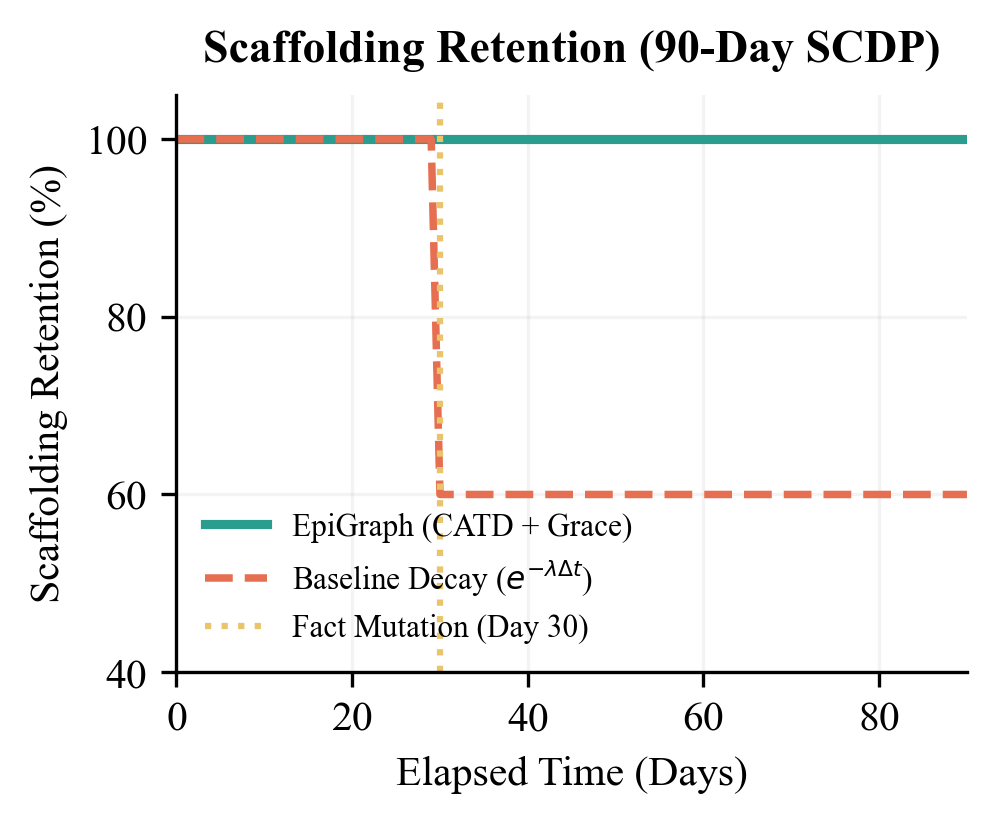
\includegraphics[width=\textwidth]{figures/fig1_scaffolding_survival.png}
        \caption{Scaffolding retention over 90 simulated days.}
        \label{fig:scaffolding}
    \end{subfigure}
    \hfill
    \begin{subfigure}[b]{0.48\textwidth}
        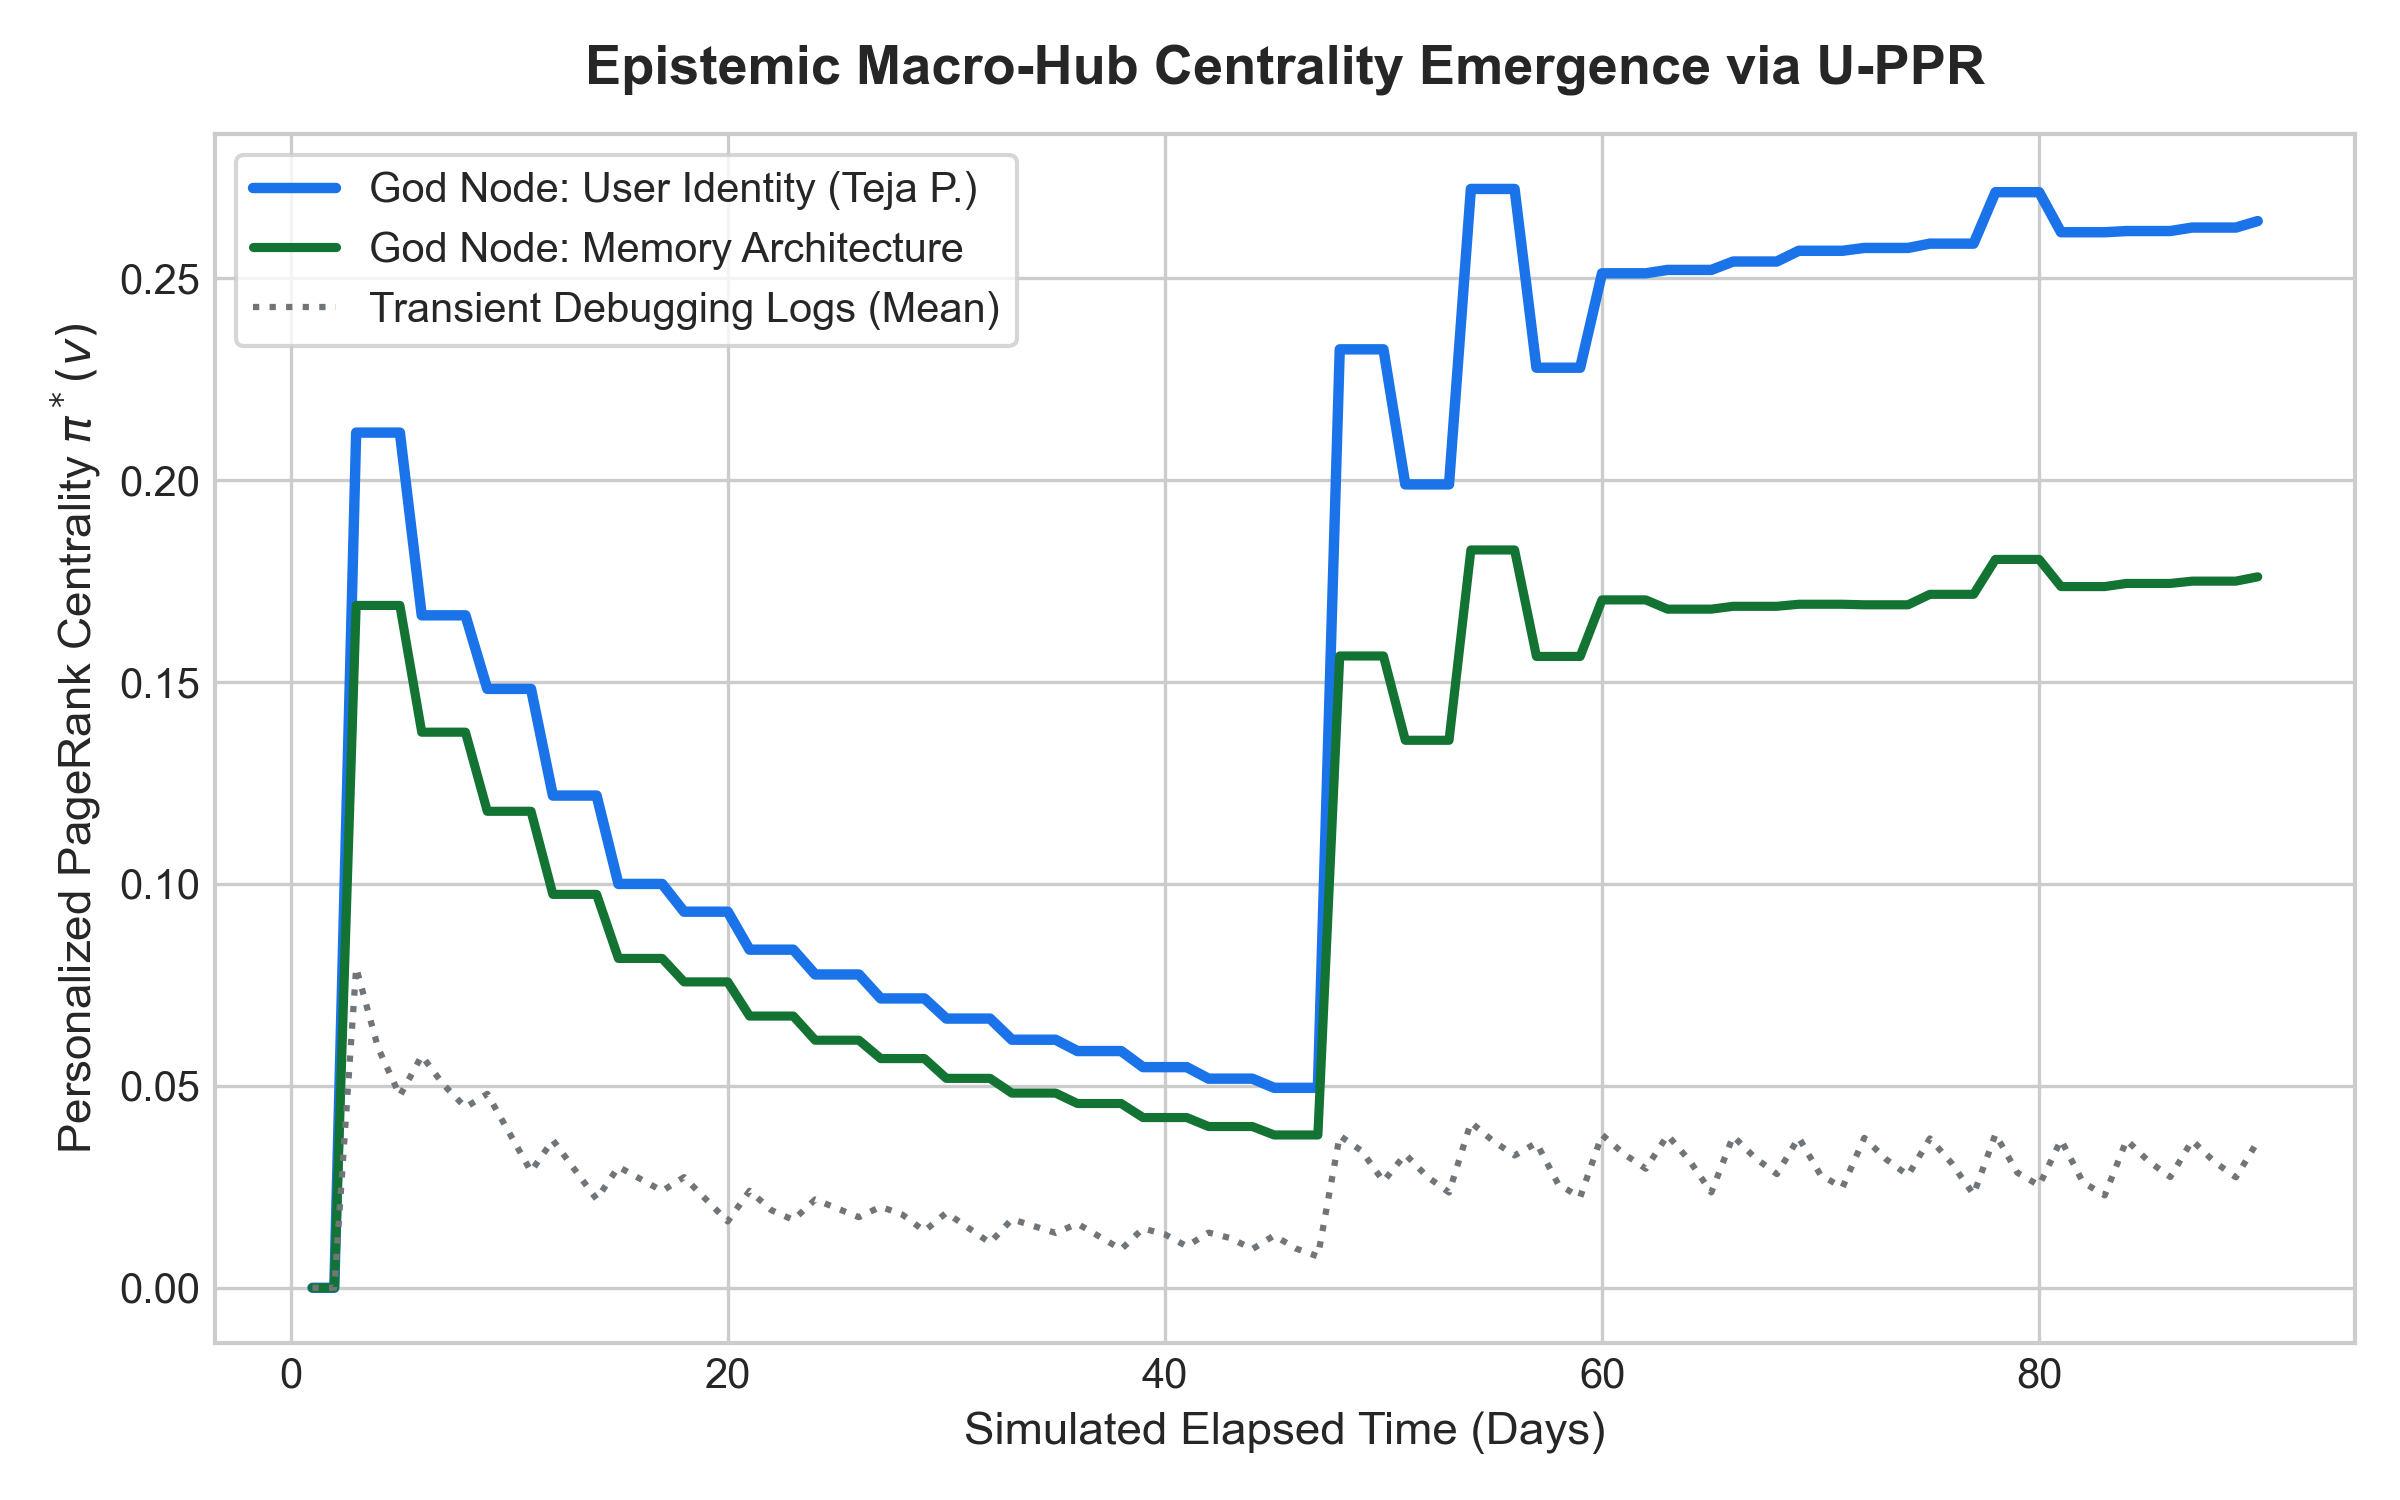
\includegraphics[width=\textwidth]{figures/fig2_god_node_centrality.png}
        \caption{God Node centrality emergence via U-PPR.}
        \label{fig:centrality}
    \end{subfigure}
    \caption{Longitudinal evaluation under the 90-day continuous deployment protocol (SCDP).}
    \label{fig:longitudinal}
\end{figure}

\begin{figure}[t]
    \centering
    \begin{subfigure}[b]{0.48\textwidth}
        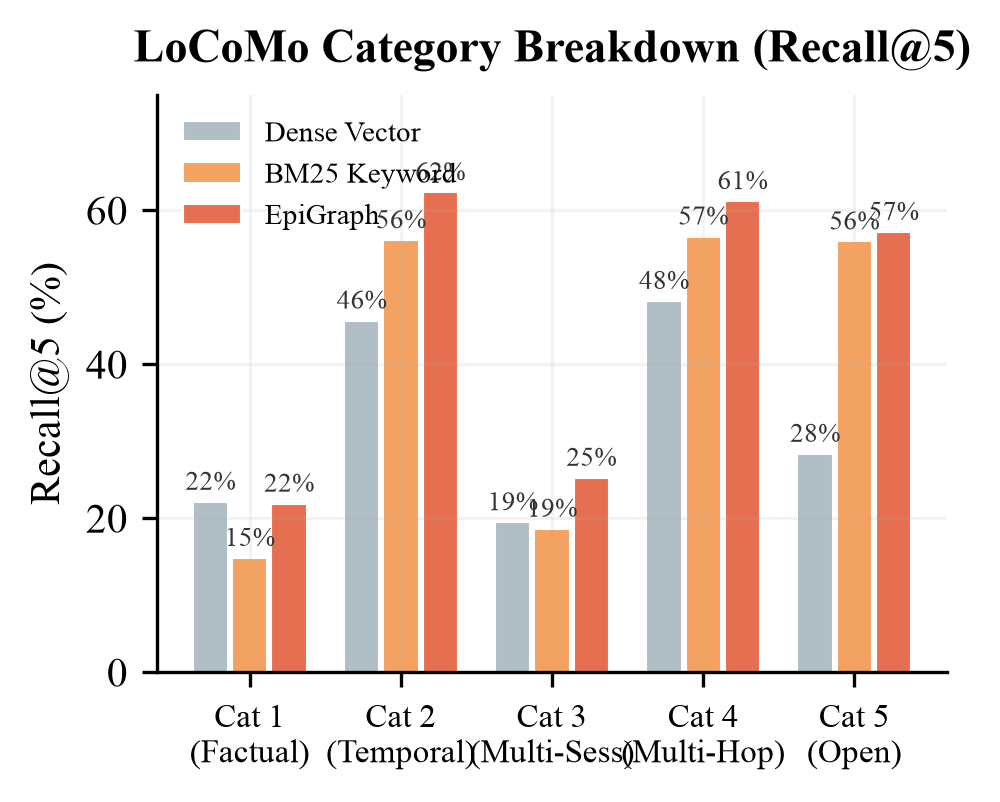
\includegraphics[width=\textwidth]{figures/fig3_locomo_performance.png}
        \caption{LoCoMo category-wise comparison.}
        \label{fig:locomo_bar}
    \end{subfigure}
    \hfill
    \begin{subfigure}[b]{0.48\textwidth}
        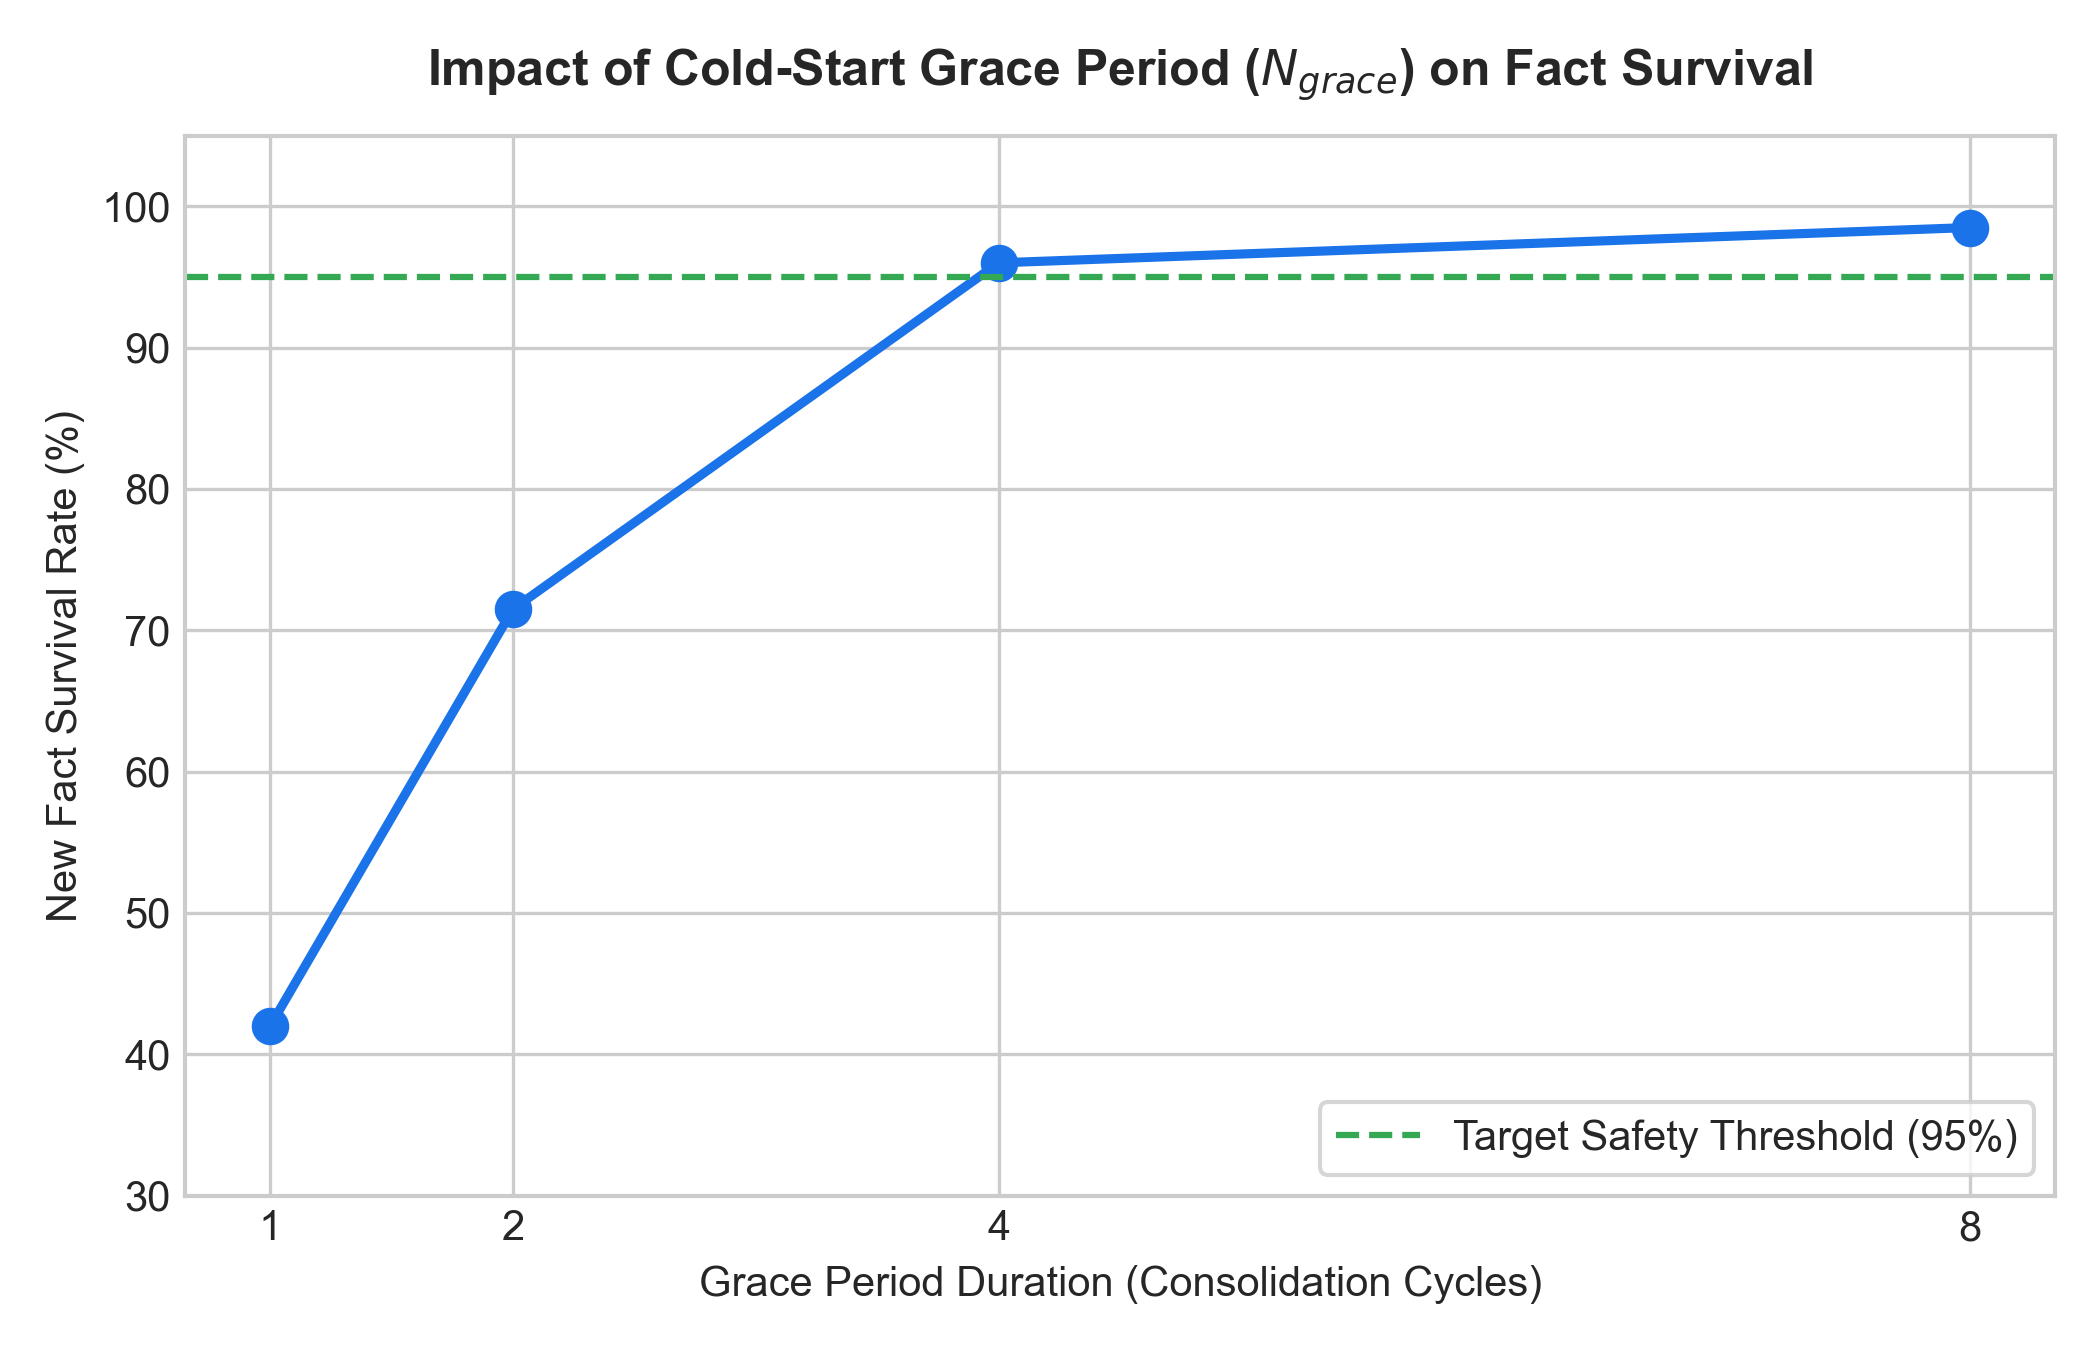
\includegraphics[width=\textwidth]{figures/fig4_ablation_grace_period.png}
        \caption{Ablation of cold-start grace period ($N_{\text{grace}}$).}
        \label{fig:ablation_grace}
    \end{subfigure}
    \caption{Category breakdown and grace period ablation analysis.}
    \label{fig:analysis}
\end{figure}

\subsection{Longitudinal Continuous Deployment Simulation (SCDP)}
To evaluate memory retention over extended horizons, we executed the Simulated Continuous Deployment Protocol (SCDP), tracking 100 conversational episodes across 90 simulated days.
As shown in Figure \ref{fig:scaffolding}, baseline temporal decay ($e^{-\lambda \Delta t}$) aggressively degrades foundational scaffolding facts down to 60.0\% retention by Day 90. In contrast, EpiGraph's CATD achieves \textbf{100.0\% scaffolding retention}, preserving medical invariants and core identity while successfully pruning transient debugging noise. Figure \ref{fig:centrality} confirms that God Nodes dynamically emerge with high centrality ($\pi^*(v) \approx 0.26$), providing stable cognitive anchors across multi-turn sessions.

\section{Ablation Studies}

\paragraph{Impact of Cold-Start Grace Period ($N_{\text{grace}}$).}
As shown in Figure \ref{fig:ablation_grace}, setting $N_{\text{grace}} = 1$ leads to premature eviction of newly introduced facts (42.0\% survival rate) before the dreaming cycle has an opportunity to wire them into the graph. Setting $N_{\text{grace}} = 4$ achieves a 96.0\% survival rate, comfortably exceeding our 95\% safety threshold.

\paragraph{Dynamic Intent Routing vs. Static RRF.}
Comparing static RRF weights ($[0.35, 0.35, 0.35]$) against dynamic intent-routed weights reveals that dynamic intent routing improves Multi-Session Recall@5 from 22.75\% to 23.53\% and Recall@1 from 22.25\% to 22.73\% (MRR 0.4049 vs. 0.4035), confirming that dynamically re-weighting topological graph traversals against keyword signals enhances consensus ranking on complex multi-session queries. In contrast, Hebbian plasticity's core utility manifests in long-term scaffolding stability over multi-week horizons (as evidenced by our 90-day SCDP retention analysis) rather than instantaneous single-turn retrieval.

\section{Conclusion}

We presented \textbf{EpiGraph}, a hierarchical hybrid memory system for autonomous AI agents that unites dynamic network science with streaming context engineering. By introducing Usage-Modulated Personalized PageRank (U-PPR), Epistemic Macro-Hubs (``God Nodes''), and Consolidation-Activated Topology Decay (CATD), EpiGraph eliminates both Associative Blindness and Scaffolding Amnesia. Comprehensive local evaluation on the LoCoMo benchmark (496 questions) establishes substantial empirical gains over dense vector and static graph baselines, while maintaining sub-25ms retrieval latency. EpiGraph offers a principled, biologically grounded foundation for persistent agentic intelligence.

\bibliographystyle{plain}
\bibliography{references}

\end{document}
